\chapter{\mFourL: A measurement designed for re-interpretation}
\label{chap:fourlepton}

\chapterquote{Very inspiring quote}
{Very inspiring quote author}

%% m4l motivation
\section{Motivation for the \mFourL measurement}
\label{sec:fourlepmotivation}

The four lepton channel is a particularly interesting channel to study as it receives contributions from many physics processes.  

First and foremost, there is the production of a pair of \PZ-bosons via quark-antiquark interactions in \info[]{s-channel not in SM because it includes neutral ZZZ or ZZ\photon vertex} both the \Ptop- and \Pup-channel. The \Ptop-channel diagram is shown in Figure \ref{fig:m4lfeynman:qqZZ}, and represents, by far, \improvement[]{Read more about why the u-channel diagram is not preferred} the largest contribution to the \ZZ production and thus to the \mFourL distribution. At the low mass end where $\mFourL=m_{PZ}$, there is resonant production of a single \PZ boson via the s-channel diagram in Figure \ref{fig:m4lfeynman:singleZ}. At $\mFourL=\unit{180}{\GeV}$ and beyond, the threshold for the on-shell production of two \PZ bosons is reached and results in a peak in the four lepton invariant mass spectrum. 

Second in magnitude is the gluon-induced production of a \PZ boson pair. This occurs via a triangle or box quark loop, which results in a factor $\alpha_s^2$ suppression. It still plays a substantial role, however, because at small $x$\footnote{Here $x$ is the component of the proton's momentum carried by the struck quark. At the \LHC the protons have very high energies; therefore the \LHC can be described as a small $x$ collider \cite{zotov2012small}} gluon-gluon luminosity is higher than the quark-antiquark luminosity \cite{Glover:194539}. The contribution from this process in on the order of ten percent \cite{Becker:2230817}. Finally in the pool of \PZ boson pairs there is a small contribution from decaying Higgs bosons, which themselves are produced also via gluon fusion, as illustrated in Figure \ref{fig:m4lfeynman:ggHZZ}. There is resonant Higgs production at \mFourL=\unit{125}{\GeV}, and a non-resonant enhancement at $\mFourL=m_{\Ptop}=\unit{350}{\GeV}$ from the top quark loop. Beyond \unit{350}{\GeV}, the Higgs-mediated \PZ boson pair production process destructively interferes with continuum production of on-shell \PZ bosons \cite{Campbell_2016}.

The \mFourL distribution can be a useful probe for certain new physics scenarios. Take for example, the high mass tail of the invariant mass spectrum. This region is dependent on the couplings of the Higgs to incoming and outgoing particles while independent of the Higgs boson width \cite{Campbell_2016}, a unique property that can be exploited to derive model-independent limits on the Higgs couplings, and on the \todo{reword, this is copy pasted} contribution of new states in the Higgs to gluon coupling \cite{Cacciapaglia_2014}. It has also been previously exploited to derive model-independent constraints on the Higgs boson width \cite{Caola_2013}. 

%% Secondly, under specific assumptions a class of models exists for which the off-shell coupling measurement together with a measurement of the on-shell signal strength can be re-interpreted in terms of a bound on the total Higgs boson width. In this paper, we provide a first step towards a classification of the models for which a total width measurement is viable and we discuss examples of BSM models for which the off-shell coupling measurement can be important in either constraining or even discovering new physics in the upcoming LHC runs

\begin{figure}
    \centering
    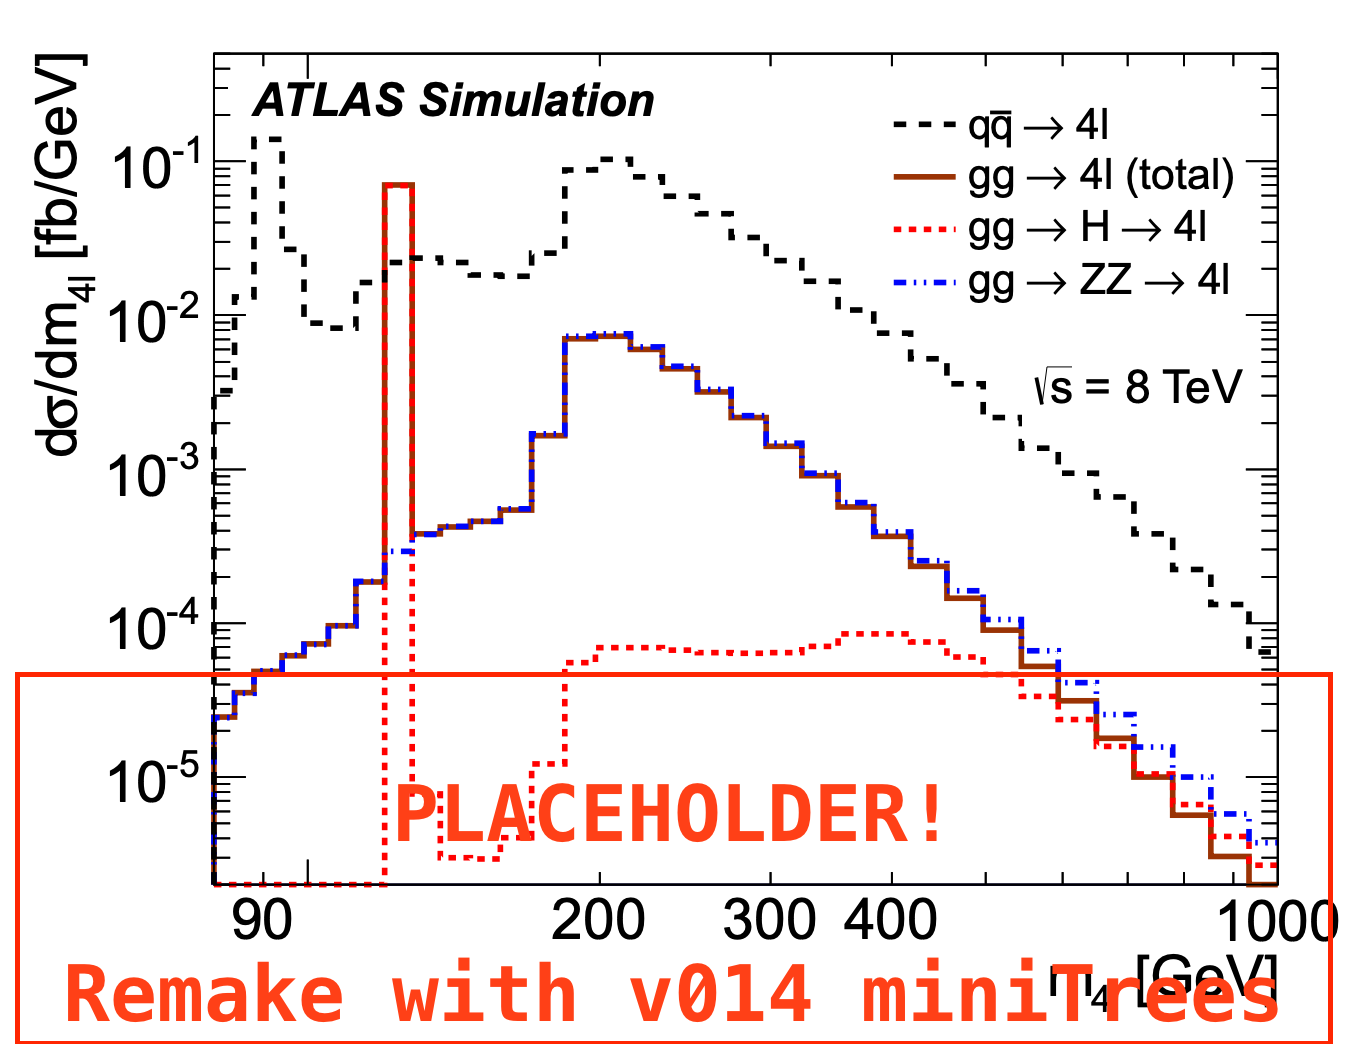
\includegraphics[width=0.5\textwidth]{Figures/m4l/m4lbreakdown.png}
    \caption{Breakdown of contributing processes contributing to the \mFourL distribution.}
    \todo[inline]{Replace and remake with our miniTrees.}
    \label{fig:m4lbreakdown}
\end{figure}

\begin{figure}
\centering
\begin{subfigure}{.24\textwidth}
  \centering
  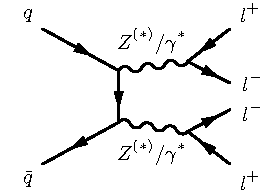
\includegraphics[width=.23\textwidth]{Figures/FeynGraphs/qqZZ4l.pdf}
  \caption{\qqZZ}
  \label{fig:m4lfeynman:qqZZ}
\end{subfigure}%
\begin{subfigure}{.24\textwidth}
  \centering
  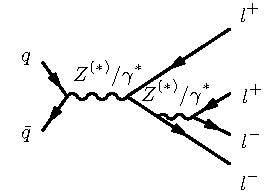
\includegraphics[width=.23\textwidth]{Figures/FeynGraphs/qqZZ4lrad.pdf}
  \caption{A subfigure}
  \label{fig:m4lfeynman:singleZ}
\end{subfigure}
\begin{subfigure}{.24\textwidth}
  \centering
  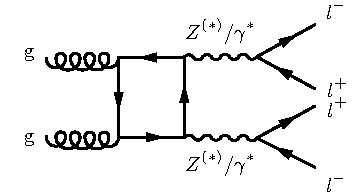
\includegraphics[width=.23\textwidth]{Figures/FeynGraphs/ggZZ4lbox.pdf}
  \caption{A subfigure}
  \label{fig:m4lfeynman:ggZZ}
\end{subfigure}
\begin{subfigure}{.24\textwidth}
  \centering
  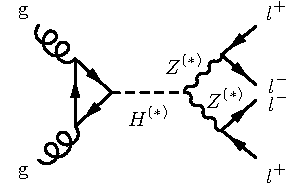
\includegraphics[width=.23\textwidth]{Figures/FeynGraphs/ggZZ4lhiggs.pdf}
  \caption{A subfigure}
  \label{fig:m4lfeynman:ggHZZ}
\end{subfigure}
\caption{Feynman diagrams for quark- and gluon-induced \ZZ production. The processes shown are the main contributors.}
\label{fig:m4lfeynman}
\end{figure}

% this channel provides a clean leptonic final state resulting in a small instrumental background, where one or more of the reconstructed lepton candidates originate from the misidentification of jet fragments or from nonprompt leptons.

%% Theoretical predictions 
\section{Theoretical predictions}
\label{sec:theory}

Theoretical predictions from Monte Carlo simulations

%% Signal definition and event selection
\section{Signal and fiducial region definition}
\label{sec:signaldef}

The motivation behind this analysis is to make a measurement as inclusive and as model-independent as possible. Any process leading to a final state of four lepton - made up of two same flavour opposite sign electron or muon pairs - is considered to be part of the signal. Electrons or muons originating from fully leptonic decays of taus are counted towards the signal. 

The fiducial region definition follows closely the acceptance of the detector. Furthermore, by loosening the mass cuts, there is higher event acceptance especially in the low mass regions. Preliminary studies were conducted to investigate the impact of loosening and simplifying the dilepton lower mass cut to \unit{5}{\GeV} and removing the upper mass cut, for example, as opposed to the varying higher cuts in the previous round of the analysis. Unsurprisingly, these result in a higher event yield in both the low and high mass tails of the \mFourL distribution. 

The final state is defined solely in terms of final state particles as opposed to targeting a specific process. Beyond the requirement of two same flavour opposite sign lepton pairs, the measurement is inclusive to additional particles such as additional leptons, jets, and invisible particles. Previous irreducible backgrounds (\VVV, \ttZ) are now considered as part of the signal since they produce four or more prompt leptons.

\missingfigure{Emily plots for loosening mass cuts}

\subsection{Lepton definitions}

For particle physicists, a prompt lepton simply means the lepton did not originate from a hadron. Prompt leptons are further classified into three categories depending on their association with emitted photons. These three categories are:
\begin{itemize}
    \item Born leptons: leptons prior to QED Final State Radiation (FSR);
    \item Bare leptons: leptons after QED FSR;
    \item Dressed leptons: leptons after QED FSR, that then have the four momenta of nearby radiated photons added to it. 
\end{itemize}
The ATLAS detector makes lepton measurements after QED FSR has occurred. It is for this reason that born leptons are not the best choice. It is more realistic to perform measurements involving only final state particles, and objects constructed from final state particles, such as dressed leptons \cite{Kar:ab1be6}. 

\subsubsection{Dressed electrons and bare muons}

In this analysis, a choice of dressing electrons but leaving muons bare was made to closer mimic what is seen by the detector. 

\subsection{Fiducial region}

\begin{table}[bp]
  \begin{tabular}{lllll}
        & Lepton requirements \\
        \midrule
        Electrons & \pt > \unit{5}{\GeV}\\
                & $|\eta| < 2.47$\\
        Muons & \pt > \unit{7}{\GeV}\\
            & $|\eta| < 2.7$\\
        \bottomrule
        \toprule
        & Event requirements \\
        \midrule
        blah & blah\\
  \end{tabular}
  \caption{Fiducial region definition.}
  \label{tab:fidregion}
\end{table}

\missingfigure[]{Dressed electrons, bare muons plot}

\section{Measured observables}

The star observable of the analysis is none other than the four lepton invariant mass, \mFourL. It has been measured previously by both the \ATLAS and the \CMS experiment \todo{missing citation} \cite{}. As with the previous round of the analysis, the \mFourL distribution is also measured double-differentially, in slices of the transverse momentum of the four lepton system, the absolute rapidity of the four lepton system, and the flavour channel of the four lepton system. 

New to this round of the analysis is the division of the four lepton invariant mass spectrum into four separate regions, each dominated by a different process. From \unit{60}{\GeV}-\unit{100}{\GeV} resonant single \Z production reigns, similarly the \unit{120}{\GeV}-\unit{130}{\GeV} region is dominated by Higgs production, and the high mass region from \unit{180}{\GeV}-\unit{2000}{\GeV} by on-shell \ZZ production. Lastly to fill the gaps between  \unit{20}{\GeV}-\unit{60}{\GeV}, \unit{100}{\GeV}-\unit{120}{\GeV}, and \unit{130}{\GeV}-\unit{180}{\GeV} is the off-shell \ZZ region. This is summarised in Table \ref{tab:m4lregions}. The following variables are measured double differentially in these four regions:

\begin{itemize}
    \item Cosine of angle $\theta^{*}$, where $\theta^{*}$ is the angle between the \todo{definitely check this} lepton in the rest frame and the \Z boson in the lab frame. This angle is sensitive to the polarisation of the decaying boson.
    \item The difference in rapidity between the lepton pairs
    \item The difference in azimuthal angle between the lepton pairs, and between leading leptons
    \item The invariant mass of the lepton pairs
    \item The transverse momentum of the lepton pairs
\end{itemize}

\begin{table}[bp]
  \begin{tabular}{lllll}
        Region & \mFourL interval(s) \\
        \midrule
        \ZFourL & \unit{60}{\GeV} < \mFourL < \unit{100}{\GeV} \\
        \HFourL & \unit{120}{\GeV} < \mFourL < \unit{130}{\GeV} \\
        On-shell \ZZ & \unit{180}{\GeV} < \mFourL < \unit{2000}{\GeV} \\
        Off-shell \ZZ & \unit{20}{\GeV} < \mFourL < \unit{60}{\GeV}, \unit{100}{\GeV} < \mFourL < \unit{120}{\GeV}, \\
           & and \unit{130}{\GeV} < \mFourL < \unit{180}{\GeV}\\
  \end{tabular}
  \caption{The four \mFourL regions dominated by the single \Z, Higgs, on-shell and off-shell \ZZ processes.}
  \label{tab:m4lregions}
\end{table}



\section{Event reconstruction and selection}
\section{Background estimation}
\label{sec:background}

\subsection{Defining leptons}

The four lepton channel is quite the golden channel, as it has a very clean signature with minimal background. In fact, the single dominant background in this analysis is when one or more of the reconstructed leptons in the quadruplet are not real leptons; rather they are misidentified objects in the detector mimicking the same signature \cite{varnes2016poisson}. These "leptons" are non-prompt, and can be referred to as a fake lepton, whereas a lepton produced from the hard scatter is a prompt, real lepton. One source of fake leptons is from hadron decays. In the case of the electron, photon conversion and hadronic jets misidentified due to their large and narrow deposit in the electromagnetic calorimeter can also play a role. In this analysis, around three-quarters of the fakes originate from \Pbottom-hadron decays in \Z plus jets and \Ptop\APtop events. 

The size and behaviour of the fake lepton background - also referred to as the reducible background - are usually estimated using data-driven methods because they are not well modelled by simulation \cite{varnes2016poisson}. One such method is the Fake Factor method. This method depends on two sets of lepton criteria: a tight criteria that selects leptons which make it into the signal region, and a loose criteria that is similar but less restrictive. The leptons selected by the latter are referred to as baseline leptons, and the baseline leptons that additionally pass the tight criteria are the signal leptons. The rest of this section will also touch on baseline-not-signal leptons; these are leptons that pass the "baseline" loose selection, but do not make the "signal" tight selection. 

\subsection{Fake Factor method}

The Fake Factor method relies on the calculation of a fake efficiency, $f$, which is the fraction of fake baseline leptons pass the tight selection criteria and become signal leptons. Because fake leptons not well modelled in simulation, the fake efficiency is calculated in data, in an alternative region of phase space that is enriched with fake leptons. 

Using the Fake Factor $F$, the number of baseline leptons, and the number of real baseline leptons, the number of fake signal leptons can be calculated. Note that the FF method assumes good modelling in the real component of the simulation since $N^{\text{baseline}}_{\text{real}}$ is taken from MC.

$$N_{\text{fake}}^{\text{signal}} = F(N^{\text{baseline}}-N^{\text{baseline}}_{\text{real}})$$

%% Smoothing

Smoothing on the raw output of the reducible background estimate is performed. The raw output, due to low statistics in certain bins, have pronounced, jagged features that resemble resonances. Of course, resonant peaks should not exist. The smoothing procedure is therefore used to obtain a more even shape, minimising the impact of any outlier bins that had a large Fake Factor weight. In order to smooth the distribution, an intermediate, finer binning is assigned to each observable and the background estimate is run. The fine-binned intermediate background distribution is smoothed with Friedman's super smoother. Lastly, the final background estimate is obtained by integrating over the smoothed distribution using the coarser, original binning. A visualisation of the process is shown in Figure \ref{fig:backgroundsmoothing}.

\missingfigure[background smoothing]

\section{Systematic uncertainties}
\label{sec:sysuncert}

\subsection{Experimental uncertainties}

Lepton (electron an muon) identification, reconstruction and isolation efficiencies.
Trigger efficiency.
Lepton momentum and scale uncertainties.
Pile-up rescaling.
Luminosity.

\subsection{Theoretical uncertainties}
QCD scale uncertainties.
PDF uncertainties.
Parton shower.
EW NLO reweighting.

%% Unfolding and respective studies
\section{Correcting for detector effects}
\label{sec:unfolding}

To unfold a measurement means to correct it for detector-effects, since what the detector sees is not what truly occurs in nature. Rather, data at the detector-level include additional side effects that one must consider, such as resolution effects, detector acceptance, etc. On the simulation side, detector simulations are the most computationally expensive. For re-interpretation purposes, having to run through the entire detector simulation chain for every model of interest is highly inefficient. Furthermore as detector technology advances and changes, as does the simulation software. In order to re-interpret detector level data published in a certain year, one would have to use the simulation software corresponding to what was in use back then. 

It is desirable to unfold Standard Model measurements so that it can be used and compared to theoretical predictions in years to come. By presenting measurements at the particle level, no further simulation is require beyond the raw output of the event generator, which is a big advantage. 

\subsection{Unfolding methodology}
\label{subsec:unfmethod}

\subsection{Binning optimization}
\label{subsec:binningopt}

The binnings of the measured distributions were optimized based on two factors: the number of events and the purity of each bin. Here the purity refers to the diagonal of the migration matrix normalised along truth, thus representing the fraction of truth events that end up in the same reconstructed event bin. There were several iterations of the binning that were run with varying criteria, summarised in table \ref{tab:BinningVersions}.

The first iteration of the binnings were run with the Default criteria. Here, depending on the number of events in the bin, the purity requirement varies. Bins with lower statistics have a high purity requirement to reduce bin-to-bin migrations. The minimum number of events required for each bin is 10. Between 10 and 15 events, the purity was required to be at least 80\%. Between 15 and 20 events the purity must be 70\% or higher. Finally for bins with more than 20 events the purity cut was 60\%. 

The binning algorithm is as follows. For the full \mFourL differential mass distribution from \unit{20}{\Gev} - \unit{2000}{\GeV}, the distribution was first split into very fine steps of \unit{1}{\GeV} bins from \unit{20}{\Gev}-\unit{450}{\GeV}. From \unit{450}{\Gev}-\unit{2000}{\GeV} wider steps of \unit{5}{\GeV} bins were used. Due to the fine nature of the bin widths, this initial binning failed to meet any of the binning criteria. Next, the binning algorithm starts from the low mass end and starts to merge adjacent bins together if the criteria were not met. For example, if bin number 1 [20,21] has > 10 events, the algorithm merges bin number 1 with the next bin. The new bin number 1 is now [20,22]. Once again, if this bin has > 10 events, it will merge again and become [20,23], and so on and so forth until 10 events has been reached. Of course the purity must also pass the required percentage for the number of events in the bin, otherwise further bin merging occurs.  

Next we have the \mFourL distributions in double differential slices of \ptFourL, \yFourL, and flavour channel. For these distributions, the fine binning is defined as the the binning of the full \mFourL differential mass distribution, i.e. the output of the algorithm described in the previous paragraph. Bins were once again checked for number events and purity, and merged as needed. This was implemented so that all \mFourL in each of the  \ptFourL, \yFourL, and flavour slices would have bin edges that match with the inclusive distribution. 

For the distributions measured double differentially in the four \mFourL regions corresponding to \Z, \Higgs, On-shell \ZZ, and Off-shell \ZZ, the same procedure was followed for binning optimisation. Each distribution had a fine binning defined, and the bins were merged from left to right of the x-axis until the criteria were met. 

\begin{table}[bp]
  \begin{tabular}{lllll}
                & Default              & Stringent              & High statistics             \\
    \midrule
                                & 10 (purity > 0.8)   & 14 &   \\
     Minimum number of events & 15 (purity > 0.7) & 20 & 100    \\
                                &20 (purity > 0.6) & 25 &    \\
  \end{tabular}
  \caption{Three different versions of binning with varying criteria.}
  \label{tab:BinningVersions}
\end{table}

\subsection{Pre-unfolding weights}
\label{subsec:preuf}



\subsection{Injection tests}
\label{subsec:injection}


\section{Results}
\label{sec:results}

Results plots